% Drawing 150/02-1 -- folder 150, batch 02, archive page 28 (PDF page 29).
% Transcription: À droite, un croquis : un coin de carré (deux axes), une courbe au-dessus et une demi-droite hachurée issue du sommet.
% Kind: corner of a square with a curve and a hatched half-line. Method 2 (schematic redraw from the facsimile). Status: ok.
% Notes: Two axes forming a corner, a wavy curve above joining their ends (doubled in places), and a half-line from the vertex with hatching beneath it.
% Coordinates: 1 unit = 1 mm = 1/100 of the crop width (bbox in page fractions: [0.45, 0.1, 0.78, 0.24]).
% Redrawn by Claude (claude-opus-5-5), issue #73, 2026-11-07; not checked by a human; not compiled (no TeX in the session).
% Rights: reproduces part of the work -- behind RENDER_TRANSCRIPTS, never published by itself.
\documentclass[tikz,border=3pt]{standalone}
\usepackage{amsmath,amssymb}
\usetikzlibrary{patterns,arrows.meta}
\tikzset{pencil/.style={black!45}, struck/.style={black!35}, mark/.style={circle,draw,inner sep=1.3pt}, pt/.style={circle,fill,inner sep=0.9pt}, opt/.style={circle,draw,fill=white,inner sep=1.1pt}}
\begin{document}
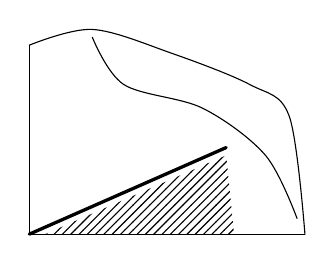
\begin{tikzpicture}[x=1mm,y=1mm,line cap=round,line join=round,font=\scriptsize]
\draw (24,-26) -- (24,-50) -- (59,-50);
\draw plot[smooth, tension=0.55] coordinates {(24,-26) (32,-24) (42,-27) (52,-31) (57,-35) (59,-50)};
\draw plot[smooth, tension=0.55] coordinates {(32,-25) (36,-31) (46,-34) (54,-40) (58,-48)};
\draw[very thick] (24,-50) -- (49,-39);
\fill[pattern=north east lines] (26,-50) -- (49,-40) -- (50,-50) -- cycle;
\end{tikzpicture}
\end{document}
